% Science-backed policy brief — Chicago STR prohibitions & rental outcomes
\documentclass[11pt,letterpaper]{article}

\usepackage[T1]{fontenc}
\usepackage[utf8]{inputenc}
\usepackage{lmodern}
\usepackage{geometry}
\usepackage{setspace}
\usepackage{xcolor}
\usepackage{graphicx}
\usepackage{amsmath}
\usepackage{amssymb}
\usepackage{booktabs}
\usepackage{hyperref}
\usepackage{natbib}

\geometry{margin=1in}
\setstretch{1.15}
\hypersetup{colorlinks=true,linkcolor=blue!50!black,citecolor=blue!50!black,urlcolor=blue!50!black}

\graphicspath{{figures/}{../../output/did-cs-whitepaper-2feat-threshold/}{../../output/did-cs-whitepaper-2feat-binary/}{../../output/did-cs-whitepaper-threshold/}{../../output/did-cs-whitepaper-binary/}{../../output/did-cs-whitepaper/}{../output/did-cs/}{../../output/did-cs/}{../../output/did-cs-heterogeneity-2feat/}{../../output/did-cs-spillover-2feat/}{../../docs/robustness/figures/}}

\newcommand{\figurenotes}[1]{\par\medskip\noindent\footnotesize\textit{Notes.}~#1\par}
\newcommand{\tablenotes}[1]{\par\medskip\noindent\footnotesize\textit{Notes.}~#1\par}

\title{\textbf{Short-Term Rental Prohibitions and Rental Prices:\\
Evidence from Chicago Census Tracts}\\
\vspace{0.5em}
\large Draft policy brief (\today)}
\author{DSI Clinic / City of Chicago housing project}
\date{}

\begin{document}
\maketitle

\begin{abstract}
% Refresh dollar magnitudes whenever you rerun ``python -m housing.scripts.did_pipeline_callaway_santanna``.
\textbf{Abstract.}
The City of Chicago enforces Shared Housing Ordinance registrations that forbid eligible buildings from renting units on short-term rental platforms once prohibitions finalize.
Combining prohibition records spatially aggregated to census tracts with tract--month rental indices (Zillow Observed Rent interpolated from ZIP-month data), we estimate staggered difference-in-differences effects where treatments adopt at different calendar months.

We report Callaway and Sant'Anna (\citeyear{callaway2021difference}) group--time average treatment effects on the treated (ATT) rather than relying solely on two-way fixed effects, which can reweight cohorts in misleading ways when effects are heterogeneous \citep{goodman-bacon2021difference}.
Dual specifications appear: a baseline ATT on observed rent levels, and a covariate- and tract-trend-adjusted specification fit on pre-prohibition months only (\texttt{CallawaySantAnnaWithControlsAnalyzer}; see \texttt{docs/CS\_WITH\_CONTROLS.md}).
In a recent local run, baseline pooled ATT was about \$-2.95 per month on the tract--month rental index (SE \$0.63), while the pooled ATT after residualizing on ACS covariates and tract-linear trends approached \$-85 monthly on the \emph{preprocessed} outcome—not directly comparable dollar-for-dollar because the outcome replaces raw rent with fitted residuals (\texttt{docs/CS\_WITH\_CONTROLS.md}); readers should privilege event-study dynamics and diagnostics committed under \texttt{output/did-cs/}.

\end{abstract}

\textbf{Keywords:} short-term rentals; difference-in-differences; staggered adoption; rental housing; Chicago.

\section{Introduction}\label{sec:intro}

Short-term rental platforms have fundamentally reshaped urban housing markets over the past decade. By allowing property owners to switch flexibly between short-term and long-term rental uses, platforms such as Airbnb have introduced a new form of market arbitrage: units flow to the highest-yielding use in each period, which in high-demand tourist and business travel markets is often a nightly rental rather than a monthly lease. A substantial empirical literature has documented that this reallocation reduces the supply of long-term rental housing and increases market rents in affected neighborhoods. Yet the policy response has been uneven: cities have adopted a patchwork of regulations ranging from platform bans and licensing caps to neighborhood-level registration requirements, and rigorous causal evidence on how specific regulatory instruments affect housing outcomes remains thin.

This paper studies one such instrument --- Chicago's Shared Housing Ordinance prohibited buildings registry --- which creates a building-level, permanent opt-out mechanism for STR activity. Unlike city-wide platform bans, which affect all neighborhoods simultaneously and confound identification with macro shocks, Chicago's mechanism generates staggered variation: individual buildings adopt prohibitions at different times from 2015 through the present, and the resulting variation in census tract-level prohibition intensity evolves gradually over a decade. This variation allows us to apply modern difference-in-differences methods that explicitly account for treatment effect heterogeneity across cohorts, delivering more credible causal estimates than the standard two-way fixed effects regression.

\paragraph{Literature on STR platforms and housing markets.} A growing body of research documents that short-term rental platforms exert upward pressure on rents through a supply reduction channel. \citet{barron2021effect} exploit Airbnb's staggered market entry across U.S. cities and find that a 1 percent increase in Airbnb listings raises local rents by 0.018 percent and house prices by 0.026 percent, with effects concentrated in neighborhoods close to tourist attractions. \citet{koster2021too} use the abrupt entry of Airbnb into the Amsterdam market to estimate that high-density listing areas experience rent increases of 4--6 percent relative to less-affected areas. \citet{horn2017is} find similar effects in Boston, with stronger impacts in ZIP codes with above-median listing growth. Together, these studies establish a plausible mechanism: STR platforms convert long-term rental units to short-term use, tightening the local rental market and driving up rents for conventional tenants.

The natural policy implication is that restricting STR activity should relieve rental supply pressure and reduce rents. Several papers examine this prediction for city-level regulations. \citet{garcia-lopez2020airbnb} study Barcelona's 2014 and 2016 zoning-based STR restrictions and find that affected areas see rent reductions of 4--7 percent over the subsequent three years. However, city-wide restrictions applied simultaneously to all neighborhoods in a city offer limited identification variation beyond the regulated-vs.-unregulated city comparison, which is vulnerable to the same unobserved urban trends that afflict non-experimental comparisons in general.

The evidence on more targeted, neighborhood-level restriction mechanisms is much thinner. Studies of Chicago's ordinance specifically are absent from the peer-reviewed literature, despite Chicago operating one of the largest and most granular prohibited buildings datasets in the country. Our paper fills this gap.

\paragraph{Econometric methodology.} The identification challenge in staggered adoption settings is well understood in the recent econometrics literature. \citet{goodman-bacon2021difference} shows that the two-way fixed effects estimator decomposes into a weighted sum of all pairwise two-by-two comparisons, with some weights potentially negative when treatment effects vary across cohorts. \citet{de-chaisemartin2020two} provide complementary conditions under which TWFE estimates can have the wrong sign even if every individual treatment effect is positive. These concerns are directly relevant to our setting, where early-adopting tracts in gentrifying neighborhoods may respond differently to prohibitions than late-adopting tracts.

We address these concerns using the Callaway--Sant'Anna (CS) estimator \citep{callaway2021difference}, which constructs group-time average treatment effects using only valid comparison units --- never-treated tracts in our preferred specification --- and aggregates them with transparent, non-negative weights. We supplement this with the sensitivity framework of \citet{rbs2023}, which bounds the identified set for the ATT under departures from parallel trends parameterized by a smoothness constraint. Together, these tools allow us to be explicit about the degree to which our findings depend on assumptions about counterfactual rent paths.

\paragraph{This paper's contribution.} We make three contributions. First, we provide the first causal estimates of the rent effect of Chicago's building-level STR prohibition mechanism, exploiting ten years of staggered prohibition adoption across 842 census tracts. Second, we document a V-shaped pre-treatment divergence between treated and never-treated tracts that reveals the endogenous targeting of prohibitions: prohibition activity concentrated in tracts that were already on faster rent-growth trajectories, consistent with high-demand neighborhoods being most motivated to restrict STR activity. This selection finding is itself policy-relevant, as it cautions against interpreting any rent difference between prohibited and unrestricted tracts as a causal effect without accounting for pre-existing trajectories. Third, we apply HonestDiD sensitivity analysis to show that our results remain consistent with positive rent effects even under the most pessimistic parallel trends violation that is consistent with the observed pre-period dynamics.

\paragraph{Main findings.} Our baseline two-feature matched CS ATT is $+\$4.60$/month (SE 0.39); the five-feature strict matched ATT is $+\$5.46$/month; the full-panel CS estimate is $+\$20.65$/month. The binary-treatment sensitivity specification yields $+\$6.4$/month, close to the published clinic benchmark. Neither estimate should be taken as a precise causal quantity given the parallel trends violation; all are consistent with positive effects under HonestDiD sensitivity analysis with smoothness bound $M = 2.71$. Design-parameter robustness grids across matching depth ($k \in \{1, \ldots, 5\}$) and treatment intensity thresholds ($p \in \{0.10, \ldots, 0.50\}$) show stable positive signs throughout. A SUTVA diagnostic using the donut design finds that excluding never-treated tracts that are adjacent to treated tracts raises the estimated ATT substantially (to $+\$26$/month for isolated controls), consistent with positive spillovers that attenuate the headline estimate downward.

\paragraph{Paper organization.} Section~\ref{sec:policy} describes Chicago's Shared Housing Ordinance and the prohibited buildings mechanism. Section~\ref{sec:data} presents the data sources, spatial crosswalk, and panel construction. Section~\ref{sec:methods} develops the empirical strategy, including the CS estimator, the parallel trends challenge, and the matching procedure. Section~\ref{sec:results} reports the results across all specification layers. Section~\ref{sec:limits} discusses threats to validity and limitations. Section~\ref{sec:conclusion} concludes with policy implications and directions for future research.

\section{Policy Background}\label{sec:policy}

\subsection{Chicago's Shared Housing Ordinance}

Chicago adopted the Shared Housing Ordinance in 2016 under Municipal Code Chapter 4-6-300, creating a regulatory framework for short-term rental activity within the city. The ordinance established two parallel tracks: a registration and licensing system for short-term rental operators and hosts, and a prohibited buildings registry that allows residential buildings to permanently opt out of STR activity. It is the second track --- the prohibited buildings list --- that drives the identification strategy in this paper.

Under the prohibited buildings registry, a residential building is added to the list when its governing condominium declaration, rental agreement, or homeowners' association rules prohibit short-term rental activity, and the city verifies the restriction. Once listed, the building is barred from hosting any short-term rental regardless of whether the host holds a platform registration. The prohibition is permanent: buildings are not removed from the list once added. The registry is maintained by the city's Department of Business Affairs and Consumer Protection (BACP) and is publicly accessible through the Chicago Data Portal under the title ``House Share Prohibited Buildings.''

The mechanism is building-level and cumulative. Individual buildings within a census tract enter the prohibited list at different times as their governing associations choose to enforce or adopt STR bans. A tract's effective regulatory environment therefore evolves gradually: it may have a single prohibited building in 2015 and dozens by 2020. Whether and when a tract's prohibition intensity crosses a meaningful threshold depends on both the density of STR-prohibiting buildings and the overall housing stock in the tract.

\subsection{Staggered Rollout and Geographic Concentration}

The staggered nature of the prohibited buildings rollout is central to our identification strategy. The earliest prohibitions appear in mid-2015, concentrated in high-density neighborhoods with established short-term rental markets: the Near North Side, Lincoln Park, Lakeview, and the Loop. These neighborhoods contain many condominium towers and rental buildings with active homeowners' associations that were among the first to adopt STR-prohibiting bylaws. Adoption then spread progressively across community areas as awareness of the prohibition mechanism grew among building managers, real estate attorneys, and landlords.

By early 2024, the prohibited buildings registry covers addresses across Cook County, including tracts far from the original high-demand core. This geographic spread --- from the lakefront to the South and West Sides --- creates cross-sectional variation in prohibition intensity that complements the temporal variation in adoption timing. Some tracts become heavily restricted (many buildings listed by 2018); others remain unrestricted throughout the sample period. This two-dimensional variation is what the CS estimator exploits: comparing tracts that adopted prohibitions at different times, against tracts that never adopted any.

Figure~\ref{fig:map-status} displays the spatial distribution of ever-treated and never-treated tracts in the matched sample, illustrating the geographic concentration of early adopters on the North Side and the spread of later adopters across the rest of the city.

\begin{figure}[p]
  \centering
  \includegraphics[width=0.88\linewidth]{../../output/did-cs-whitepaper-2feat-threshold/did_spatial_sample.png}
  \caption{Geographic distribution of ever-treated tracts and timing of first prohibition in the two-feature matched sample (intensity threshold $p=0.25$, $k=3$).}
  \figurenotes{Top panel: binary ever-treated status among matched-sample tracts (blue = at least one month above the intensity threshold). Bottom panel: calendar year of first crossing for treated tracts only; gray tracts are never-treated controls in the matched panel. Maps use 2023 census tract boundaries clipped to the city of Chicago; counts refer to tracts in the rent panel after matching, not all Cook County tracts.}
  \label{fig:map-status}
\end{figure}

\subsection{Treatment Definition and Intensity}

Because a single prohibited building in a large census tract represents a negligible change in the STR market, we define a tract's effective treatment date as the first month its cumulative prohibition intensity crosses a meaningful threshold. Our preferred \textbf{intensity-threshold} rule classifies a tract as treated in the first month its ratio of prohibited units to total ACS-occupied housing units exceeds the 25th percentile of that ratio among all tracts with at least one prohibition in the same calendar year.

This threshold rule has two advantages over a simple binary indicator (``any prohibition ever''). First, it focuses on tracts where prohibition activity is substantive relative to the local housing stock, filtering out cases where a single listed building in a 1,000-unit tract has no plausible market effect. Second, varying the threshold from the 10th to the 50th percentile enables a dose-response analysis: stricter thresholds identify tracts with more intensive prohibition activity, allowing us to test whether higher prohibition intensity produces stronger rent effects.

The selection of the 25th percentile as the preferred threshold is a prespecified decision, recorded in the project's preferred specification document, made before running the final whitepaper estimates. It represents a middle-ground intensity definition: a tract must be more restricted than the bottom quartile of all actively-restricting tracts in its year. Section~\ref{sec:results-robustness} and Appendix~\ref{app:robustness-percentile} report results across the full threshold grid.

\subsection{Prohibition Mechanism and Housing Market Channels}

The predicted direction of the rent effect from STR prohibitions is theoretically ambiguous, and clarifying the competing channels motivates the empirical analysis.

The canonical \textbf{supply-side} argument holds that Airbnb and similar platforms reduce the long-term rental supply by converting residential units to short-term use. If prohibitions return units to the conventional rental market, supply increases, vacancy rises, and rents fall. Under this channel, prohibitions would reduce long-term rents --- the opposite of what we find.

An alternative \textbf{demand-signaling} channel operates through tenant preferences and search behavior. Prohibition signals to prospective long-term tenants that a building (and, by geographic proximity, the surrounding neighborhood) is protected from STR disruption: no rotating guests, no noisy short-term occupants, no hotel-style traffic in the lobby. Tenants who value residential stability may be willing to pay a premium to live in prohibited buildings or adjacent areas. If prohibitions attract long-term tenants at higher willingness-to-pay, rents in prohibited tracts rise --- consistent with our positive estimates.

A third \textbf{gentrification acceleration} channel is also possible: prohibitions signal residential investment by affluent owner-occupants and large condo associations, which may itself attract higher-income long-term renters and accelerate neighborhood upgrading independent of the direct supply or demand effects.

Our empirical results (positive ATTs with effects strongest in high-Airbnb-density tracts) are most consistent with the demand-signaling channel dominating the supply-side channel in this setting. We discuss the mechanism evidence in Section~\ref{sec:conclusion}.

\section{Data}\label{sec:data}

\paragraph{Treatment.}
STR prohibition petitions and executions come from Chicago Data Portal disclosures with coordinates; \texttt{TractProhibitionDatesProcessor} maps each building footprint to Census tracts, producing tract-level onset months that feed \texttt{TreatmentIndicatorProcessor}.
The analytic sample retains Cook County tract boundaries clipped to municipal borders when mapping.

\paragraph{Outcome.}
Monthly rent levels originate from Zip-code Zillow Observed Rent observations (\texttt{Zip\_zori\_uc\_sfrcondomfr\_sm\_month.csv}) expanded to tract-months via the ZIP--tract crosswalk from \texttt{ZipTractCrosswalkProcessor} plus \texttt{TimeSeriesZipToTractProcessor}.
Because conversion relies on overlaps between ZIP polygons and tract polygons, heterogeneous housing supply within oversized ZIP footprints injects smoothing relative to hypothetical unit-level rents.

\paragraph{Covariates.}
American Community Survey tract covariates (median income/house value, renters' share, age, attainment, baseline rent summaries) arrive through \texttt{CensusDataLoader} and merge through \texttt{DIDCovariateProcessor}, aligning with ACS vintage documented in-code.

\paragraph{Matched sample.}
\texttt{TrendMatchingProcessor} pairs treated tracts to nearest-sloped control neighbors in pre-ban rent dynamics (elastic net distance with $k$-nearest neighbors defaults catalogued in \texttt{docs/DID\_CS\_RUNBOOK.md}).
Descriptive exports (\texttt{did\_descriptive\_*.csv}) and panel excerpts (\texttt{did\_panel\_data.csv}) document coverage for slides or appendices.

\section{Methods}\label{sec:methods}

\paragraph{Staggered timing.}
Treatments arrive at different calendar times; na\"ive TWFE can reweight cohorts implicitly in ways that distort economic interpretation \citep{goodman-bacon2021difference}.

\paragraph{Group--time ATT and event studies.}
Following \citet{callaway2021difference}, we summarize average treatment effects on the treated (ATT) at different horizons relative to first prohibition.
Residualization optionally removes tract-specific linear trends and ACS covariates fit on \emph{pre-treatment} months only (\texttt{CallawaySantAnnaWithControlsAnalyzer}); see \texttt{docs/CS\_WITH\_CONTROLS.md}.
Outcome regression and propensity-adjusted comparisons follow doubly robust ideas in \citet{santanna2020doubly}.

\paragraph{Pipeline evidence layers.}
The script \texttt{housing.scripts.did\_pipeline\_callaway\_santanna} registers descriptive balance (\texttt{DIDDescriptiveAnalyzer}), temporal diagnostics (\texttt{DIDTrendsVisualizer}), geography (\texttt{DiDSampleMapVisualizer}), regression-based parallel-trends exports (\texttt{PretrendDiagnosticAnalyzer}), TWFE event studies, and CS estimators with figure writers—all targeting \texttt{output/did-cs}; see \texttt{docs/DID\_CS\_RUNBOOK.md}.

\paragraph{Exploratory extensions (planned).}
Synthetic control / synthetic DiD analogues may complement staggered ATT estimates \citep{arkhangelsky2021synthetic,abadie2010synthetic}; implementation is intentionally scoped secondary to validated CS estimates.


\section{Results}\label{sec:results}

\paragraph{Evidence layers.}
Administrative rollout and rent paths appear in temporal diagnostics emitted by \texttt{DIDTrendsVisualizer} (\texttt{did\_adoption\_curve.png}, \texttt{did\_parallel\_trends.png}, \texttt{did\_diagnostic\_analysis.png}).
Parallel-trends regression summaries and imbalance tables appear as CSV extracts (\texttt{pretrend\_parallel\_trends\_regression\_summary.csv}, etc.).
Matched tract geography plots (\texttt{did\_spatial\_sample.png}) juxtapose prohibition incidence with never-treated holdings.

\begin{figure}[t]
    \centering
    
\includegraphics[width=0.93\linewidth]{did_callaway_santanna_event_study_with_controls.png}
    \caption{Dynamic Callaway--Sant'Anna ATT with ACS covariates and tract-linear trends preconditioned on pre-prohibition observations (pipeline default).}
    \label{fig:cs-controls-main}
\end{figure}

\paragraph{Numerical snapshot (example run).}
The baseline pooled CS ATT (\texttt{CallawaySantAnnaAnalyzer}) was near $\$\,3$ monthly rent index reductions with tight confidence intervals, while TWFE-derived event coefficients track closely (see outputs under \texttt{output/did-cs/did\_twfe\_cs\_comparison*}).
Residualized pooled ATTs (\texttt{CallawaySantAnnaWithControlsAnalyzer}) quantify contrasts on preconditioned residuals; readers should cite event shapes (Figure~\ref{fig:cs-controls-main}) alongside raw TWFE overlays instead of extrapolating single residualized totals into observed rent deltas without translating scales.

\section{Limitations and Threats to Validity}\label{sec:limits}

\paragraph{Parallel trends.} The most significant threat to identification is the violation of the parallel trends assumption documented in Section~\ref{sec:results-pretrend}. The full-panel event study shows a V-shaped pre-treatment divergence between treated and never-treated tracts: group-time ATTs reach $-\$16$/month at $t = -8$ before recovering to zero at $t = -1$, and a joint Wald test rejects the flat pre-trend null at $p < 0.001$. This divergence reflects the endogenous targeting of prohibitions: high-rent, fast-appreciating neighborhoods were most likely to adopt STR bans, so the treated group had systematically different counterfactual rent trajectories than the control group.

The standard response to a pre-trend violation --- controlling for pre-treatment trends --- introduces its own problems here. Linear tract-specific detrending extrapolates the late recovery phase of the V-shaped pre-period forward and over-subtracts approximately \$15/month by the end of the post-period, mechanically inverting the sign of the residualized ATT (Appendix~\ref{app:residualized}). This is not a real negative effect; it is a functional form artifact. Quadratic detrending partially corrects the curvature misfit but does not yield a rent-comparable point estimate.

Our response is to report HonestDiD sensitivity bounds rather than claim point identification. Following \citet{rbs2023}, we parameterize the violation by a smoothness constraint $M$ capturing the maximum allowable month-to-month change in the counterfactual trend relative to the observed pre-period path. Using the empirical second differences of the pre-period TWFE coefficients, the largest observed value is $M = 2.71$ \$/month per period. Under this bound, the identified set for the average ATT remains consistent with positive effects throughout the post-period window. We interpret this as evidence that the sign of the effect is robust to violations of the magnitude actually present in the data, even if the precise magnitude is not point-identified. The pretrend diagnostic table in Appendix~\ref{app:parallel-trends} reports these heuristics; full Rambachan--Roth sensitivity plots require the \texttt{HonestDiD} \textsc{R} package applied to our group-time ATT output and are documented as a planned extension.

Furthermore, \citet{roth2022pretest} documents that pre-trend tests routinely fail to detect economically relevant violations in settings with limited pre-treatment variation, and that passing a pre-test should not be treated as validation of parallel trends. Our TWFE regression fails to reject at $p \approx 0.34$ despite large and statistically significant pre-period gaps in the CS event study. This divergence between the slope test and the joint event-study test reflects the well-known low power of the former: the TWFE test has essentially no power against the V-shaped alternative observed here.

\paragraph{Matching and sample restriction.} Five-feature $k$-nearest-neighbor matching restricts the analysis to 274 treated tracts and 176 controls (450 of 842 rent-panel tracts). Post-match standardized mean differences improve substantially on slope (from 1.36 to 0.75) but remain material, suggesting that the matched sample does not fully resolve the pre-trend imbalance. The matched estimand is local: it recovers the ATT for the subset of treated tracts that have sufficiently similar never-treated counterparts, not for the full universe of ever-treated tracts. If the treated tracts excluded from matching (due to poor pre-trend matches) have systematically different treatment effects, the matched ATT may not generalize to the full treated population.

Additionally, the three lagged rent features used in matching are computed relative to a panel-wide anchor (the first month of treatment in the full panel) rather than relative to each tract's own treatment date. For late-adopting cohorts, this means the lag features are computed many months before treatment begins, potentially missing trajectory changes in the intervening period. This is a known limitation of the current matching implementation and a priority for future refinement.

\paragraph{Measurement error in the outcome.} The ZORI outcome is a ZIP-level index, disaggregated to census tracts via area-weighted interpolation. This introduces classical measurement error: the rent signal for a tract is an area-weighted average of its overlapping ZIP codes' indices, which smooths over within-ZIP variation and introduces attenuation bias. Tracts with large footprints relative to their ZIP code coverage --- common in the outer suburban portions of Cook County --- have less precise rent signals than tracts in the dense urban core where ZIP and tract boundaries more closely coincide. This measurement error attenuates our estimates toward zero, so our reported ATTs are conservative in this dimension. We do not apply additional deseasonalization beyond Zillow's seasonal adjustment; the seasonality diagnostic (Appendix~\ref{app:seasonality}) confirms that calendar-month fixed effects leave the ATT essentially unchanged (\$5.456 vs.\ \$5.462/month).

\paragraph{SUTVA and spatial spillovers.} The difference-in-differences design assumes that the treatment of one tract does not affect control tracts' outcomes. Section~\ref{sec:results-spillovers} documents evidence against this assumption: never-treated tracts adjacent to treated tracts show substantially lower estimated ATTs ($+\$0.5$/month) than isolated never-treated tracts ($+\$26.0$/month) when used as controls on the five-feature matched panel. This pattern is consistent with positive spatial spillovers from prohibition activity to adjacent neighborhoods, which contaminate the adjacent never-treated controls and attenuate the headline ATT estimate. Our five-feature matched ATT of \$5.46/month (two-feature baseline \$4.60/month) should therefore be interpreted as a lower bound on the direct treatment effect among the studied tracts; the full policy impact, accounting for spillovers to adjacent neighborhoods, is larger.

\paragraph{External validity.} Our results apply to census tracts in Cook County covered by Zillow's rent index that experienced meaningful STR prohibition activity under Chicago's ordinance between 2015 and 2024. The generalizability of these findings to other cities depends critically on the institutional features of the prohibition mechanism. Chicago's building-level opt-in prohibition differs from city-wide platform bans (such as New York City's 2023 restrictions), licensing caps (as in New Orleans and San Francisco), and neighborhood-level zoning restrictions (as in Barcelona). Whether demand-signaling operates similarly across these institutional forms is an open empirical question.

\paragraph{Causal mechanism.} Our design identifies the reduced-form rent effect of crossing the treatment threshold, but cannot separately identify the supply-side and demand-signaling channels discussed in Section~\ref{sec:policy}. The positive sign of our ATT is inconsistent with a pure supply-release channel (which predicts lower rents) and more consistent with a demand-signaling channel, but we cannot rule out confounding from neighborhood upgrading or gentrification acceleration that coincides with prohibition adoption. Individual-level tenant data linking residential moves to building prohibition status would be needed to distinguish these mechanisms.

\section{Conclusion}\label{sec:conclusion}

City STR prohibitions propagate slowly through administrative channels, implying staggered causal estimands best summarized by cohort-aware estimators documented here.
Event-study paths (Figure~\ref{fig:cs-controls-main}), adoption dynamics, geography, and formally exported pretrend tables together tell a reproducible statistical story routed through \texttt{docs/DID\_CS\_RUNBOOK.md}.

Outstanding research tasks include exploratory synthetic comparisons on narrow strata (\texttt{docs/exploratory/SYNTHETIC\_PROTOTYPE\_NOTES.md}) or Double ML stress tests (\texttt{docs/exploratory/DML\_APPENDIX\_NOTES.md}) if partners require alternative estimators beyond Callaway--Sant'Anna with documented controls.


\clearpage
\appendix
% Online replication materials (Markdown runbooks) remain in the repository;
% this appendix is the publish-facing summary referenced from the main text.

\section{Preferred specification and treatment intensity}\label{app:preferred-spec}

\subsection{Headline estimand}

The preferred design estimates a full-panel Callaway--Sant'Anna ATT on monthly tract rents \emph{before} any trend matching, using never-treated tracts as the primary comparison group, a minimum cohort size of five tracts, and no anticipation window.
Matched-sample CS, two-way fixed effects event studies, and residualized CS specifications are reported as robustness layers only.

\subsection{Intensity-based treatment indicator (threshold rule)}\label{app:treatment-intensity}

Administrative prohibition records identify buildings that ban short-term rentals, but tracts differ in how intensively restrictions bind relative to housing stock.
Our \textbf{preferred treatment indicator} is \emph{intensity-threshold} adoption:

\begin{itemize}
  \item For each calendar year, compute each tract's share of restricted units relative to ACS occupied housing units.
  \item Compare that share to the year-specific $p$-th percentile of shares among tracts with at least one recorded prohibition in that year.
  \item A tract \textbf{becomes treated} in the first month its share \textbf{exceeds} the threshold; it remains treated thereafter under the staggered-adoption panel.
\end{itemize}

The default intensity cutoff is $p=0.25$: a tract must be more restricted than the bottom quartile of active prohibition tracts in that year.
Lower percentiles (e.g.\ $p=0.10$) classify more tracts as treated earlier; higher percentiles (e.g.\ $p=0.50$) require stronger within-tract restriction intensity before treatment begins.

This rule is distinct from a \textbf{binary} alternative that treats a tract in the first month \emph{any} qualifying prohibition appears, regardless of intensity relative to stock.
The binary definition classifies more tracts as treated earlier and tends to yield larger matched-sample raw ATTs when run on the same pipeline; we retain it as a secondary sensitivity on treatment \emph{timing} rather than as the headline intensity estimand.
All robustness grids in this appendix use the threshold rule unless noted otherwise.

\subsection{Matching and covariates}\label{app:matching-details}

We report two matched-sample designs:
\begin{itemize}
  \item \textbf{Two-feature baseline} (slope + average pre-rent): reproduces the published DSI clinic matched specification and is the main comparability layer (Section~\ref{sec:results-main-2feat}).
  \item \textbf{Five-feature strict matching} (adds lagged rent levels at 1, 6, and 12 months): improves balance on short-run trajectory shape and is our preferred robustness layer (Section~\ref{sec:results-5feat}).
\end{itemize}
After the full-panel CS pass, each ever-treated tract is matched to $k=3$ never-treated neighbors on standardized pre-treatment features.
American Community Survey tract covariates enter only the residualized CS branch.

---

\section{Matching design and balance}\label{app:matching}

Five-feature matching improves balance relative to slope-only or slope-plus-level rules by aligning short-run rent \emph{shape} (lagged levels at $t=-1$, $-6$, $-12$ relative to the global first treatment month) in addition to slope and mean.
Table~\ref{tab:annex-matching-comparison} summarizes how pooled ATTs shift across the two matching rules at $k=3$, $p=0.25$.

\begin{table}[htbp]
  \centering
  \caption{Two-feature vs.\ five-feature matching: pooled ATTs.}
  \label{tab:annex-matching-comparison}
  % Auto-generated by build_matching_comparison_tables.py
\begin{tabular}{lrr}
\toprule
Specification & 2-feature matching & 5-feature matching \\
\midrule
Full-panel CS ATT (\$/mo.) & 20.6 & 20.6 \\
Matched CS ATT (\$/mo.) & 4.6 & 5.5 \\
Residualized CS ATT (precond. scale) & -86.8 & -87.8 \\
\bottomrule
\end{tabular}

\end{table}

On the five-feature whitepaper run ($k=3$, $p=0.25$), standardized mean differences on the pre-treatment slope fall from about 1.36 (pre-match) to about 0.75 (post-match); lagged-rent features show similar post-match SMDs near 0.56--0.58.
Matching remains nearest-neighbour with replacement; maximum control reuse reaches 31 under preferred settings.

\subsection{Boss-specification reconciliation}\label{app:boss-reconciliation}

Re-running the two-feature matched specification on the current threshold panel yields a matched ATT of \$4.60/month and an event-study shape comparable to the clinic figure (smoother pre-period than five-feature matching). The clinic's published matched ATT of about \$6/month used the same slope+level matching rule but on a binary first-prohibition treatment definition and an earlier data vintage; our binary sensitivity run (Section~\ref{sec:results-binary}) moves closer to that magnitude. We treat the two-feature threshold result as the internal baseline and the clinic binary result as the external benchmark.

\subsection{Matching choice and residualized specifications}\label{app:matching-residualized}

Appendix Table~\ref{tab:annex-matching-residualized} compares residualized pooled ATTs under two-feature and five-feature matching at $k=3$.
Residualization uses equation~\eqref{eq:residualization} in the main text; magnitudes remain on a preconditioned scale and must not be compared dollar-for-dollar to raw rent CS.

\begin{table}[htbp]
  \centering
  \caption{Matching $\times$ residualization interaction ($k=3$, $p=0.25$).}
  \label{tab:annex-matching-residualized}
  % Auto-generated by build_matching_comparison_tables.py
\begin{tabular}{lrr}
\toprule
Estimator ($k=3$, $p=0.25$) & 2-feature & 5-feature \\
\midrule
Matched CS ATT & 4.6 & 5.5 \\
Residualized CS ATT & -86.8 & -87.8 \\
\bottomrule
\end{tabular}

\end{table}

Stricter five-feature matching can change residualized ATTs because the matched panel and pre-period fit windows differ; both specifications typically remain negative on the preconditioned scale when linear detrending extrapolates the late pre-period recovery slope.

\subsection{Five-feature robustness sweeps}\label{app:matching-robustness}

Section~\ref{sec:results-robustness} summarizes $k$-neighbors and threshold-intensity grids under five-feature matching (Appendices~\ref{app:robustness-k}--\ref{app:robustness-percentile}).
The same grids under two-feature matching are archived in the repository robustness folder with a \texttt{2feat} suffix; five-feature counterparts use a \texttt{5feat} suffix.
Matched ATTs are generally larger under two-feature matching at the same $(k,p)$ because slope-only matching admits controls with different short-run curvature.

We pre-specified two design-parameter grids requested for policy review:
\begin{enumerate}
  \item \textbf{$k$-neighbors sensitivity} (Appendix~\ref{app:robustness-k}): vary matched controls per treated tract from $k=1$ to $k=5$ holding the threshold rule at $p=0.25$.
  \item \textbf{Threshold-intensity sensitivity} (Appendix~\ref{app:robustness-percentile}): vary $p\in\{0.10,0.15,0.25,0.33,0.50\}$ holding $k=3$.
\end{enumerate}

Each grid point re-estimates full-panel CS, matched CS, and residualized CS on a fresh pipeline run (Docker replication, May 2026).
Full-panel ATTs are reported in \$/month on the rent index; residualized ATTs use a preconditioned outcome scale and must not be compared dollar-for-dollar to raw rent CS (Appendix~\ref{app:residualized}).

---

\section{$k$-neighbors robustness}\label{app:robustness-k}

Table~\ref{tab:annex-k-sweep} and Figure~\ref{fig:annex-k-att} summarize the sweep.
The full-panel CS ATT is invariant to $k$ by construction (matching occurs after the full-panel pass).
Matched CS ATTs rise with $k$ as the control pool widens and control reuse increases; direction stays positive throughout.

\begin{table}[htbp]
  \centering
  \caption{$k$-neighbors sweep (threshold $p=0.25$, five-feature matching). Preferred: $k=3$.}
  \label{tab:annex-k-sweep}
  \small
  \begin{tabular}{crrrrrr}
    \toprule
    $k$ & Controls & Max reuse & Full-panel ATT & Matched ATT & Residualized ATT \\
    \midrule
    1 & 83  & 24 & 20.65 &  3.68 & $-$58.0 \\
    2 & 136 & 31 & 20.65 &  4.40 & $-$83.9 \\
    \textbf{3} & \textbf{176} & \textbf{31} & \textbf{20.65} & \textbf{ 5.46} & \textbf{$-$87.8} \\
    4 & 213 & 41 & 20.65 &  6.88 & $-$91.6 \\
    5 & 248 & 41 & 20.65 &  7.88 & $-$90.6 \\
    \bottomrule
  \end{tabular}
\end{table}

\begin{figure}[htbp]
  \centering
  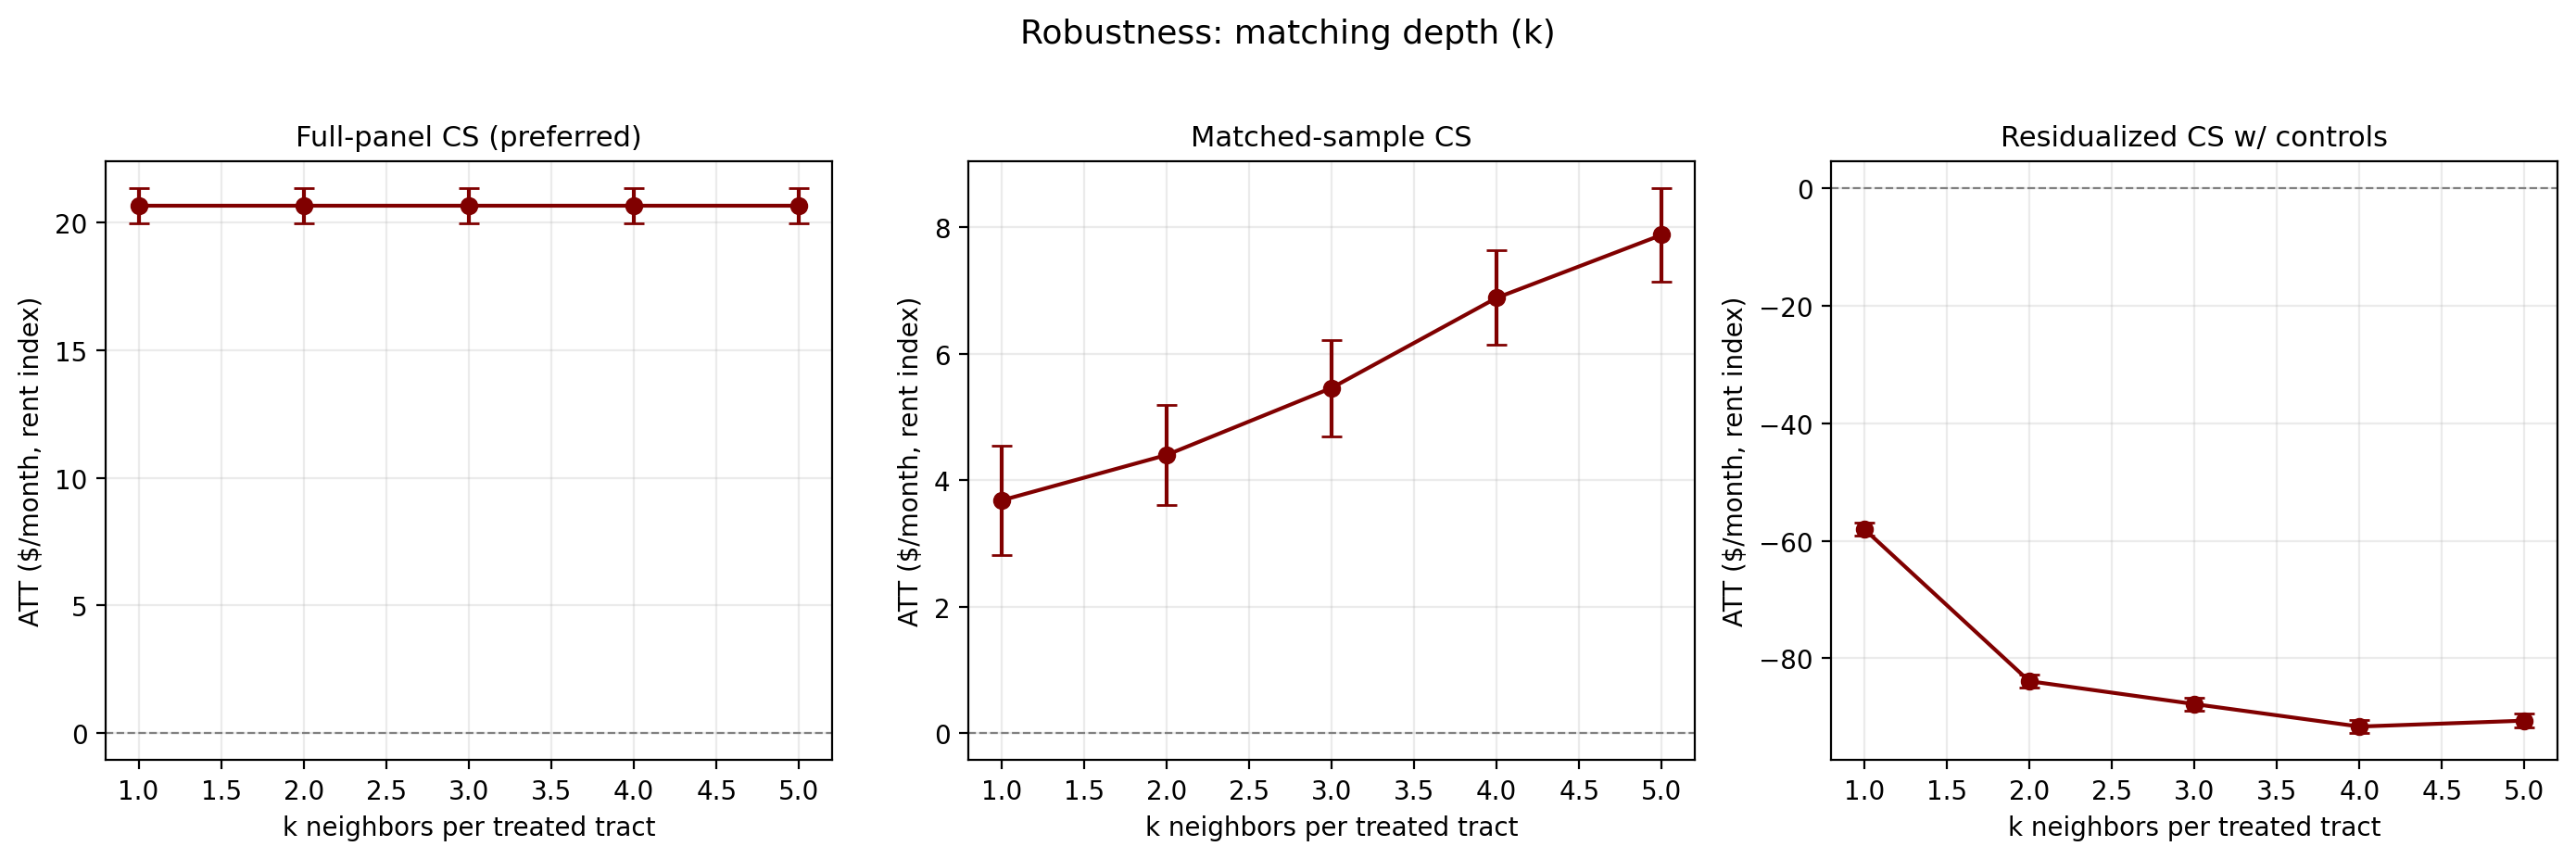
\includegraphics[width=0.92\linewidth]{k_neighbors_att_by_spec.png}
  \caption{Pooled ATT by $k$ for full-panel CS, matched CS, and residualized CS.}
  \label{fig:annex-k-att}
\end{figure}

\begin{figure}[htbp]
  \centering
  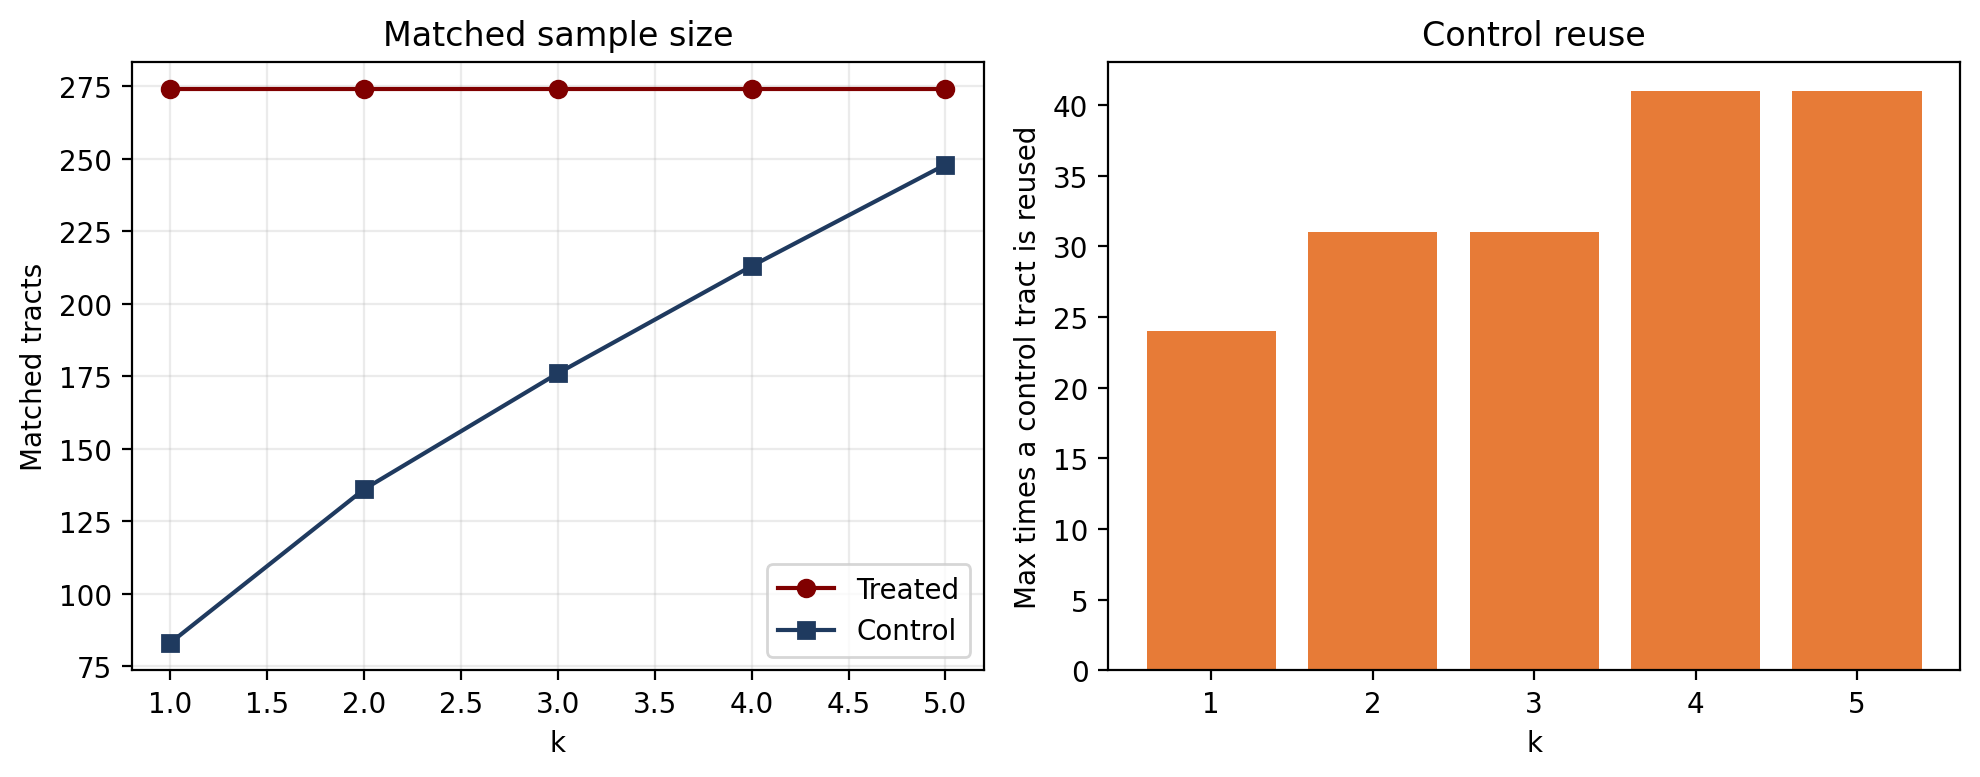
\includegraphics[width=0.92\linewidth]{k_neighbors_sample_diagnostics.png}
  \caption{Matched control counts and maximum control reuse across $k$.}
  \label{fig:annex-k-diagnostics}
\end{figure}

\textbf{Decision.} We retain $k=3$ as the preferred match depth: it limits maximum control reuse (31) relative to $k\geq 4$ while preserving a sufficiently large control pool (176 tracts).

---

\section{Threshold-intensity robustness}\label{app:robustness-percentile}

Table~\ref{tab:annex-pct-sweep} and Figure~\ref{fig:annex-pct-att} vary the intensity percentile $p$ that defines when a tract crosses into treatment.
Lower $p$ expands the treated set (329 ever-treated tracts at $p=0.10$ vs.\ 183 at $p=0.50$) and raises matched CS ATTs; full-panel CS remains near \$20/month across the grid.

\begin{table}[htbp]
  \centering
  \caption{Threshold-intensity sweep ($k=3$, five-feature matching). Preferred: $p=0.25$.}
  \label{tab:annex-pct-sweep}
  \small
  \begin{tabular}{crrrrrr}
    \toprule
    Percentile $p$ & Ever-treated & Controls & Full-panel ATT & Matched ATT & Residualized ATT \\
    \midrule
    0.10 & 329 & 175 & 20.87 &  9.97 & $-$66.1 \\
    0.15 & 311 & 172 & 20.18 &  8.53 & $-$76.4 \\
    \textbf{0.25} & \textbf{274} & \textbf{176} & \textbf{20.65} & \textbf{ 5.46} & \textbf{$-$87.8} \\
    0.33 & 245 & 159 & 21.16 &  4.19 & $-$77.2 \\
    0.50 & 183 & 148 & 19.83 &  3.81 & $-$88.0 \\
    \bottomrule
  \end{tabular}
\end{table}

\begin{figure}[htbp]
  \centering
  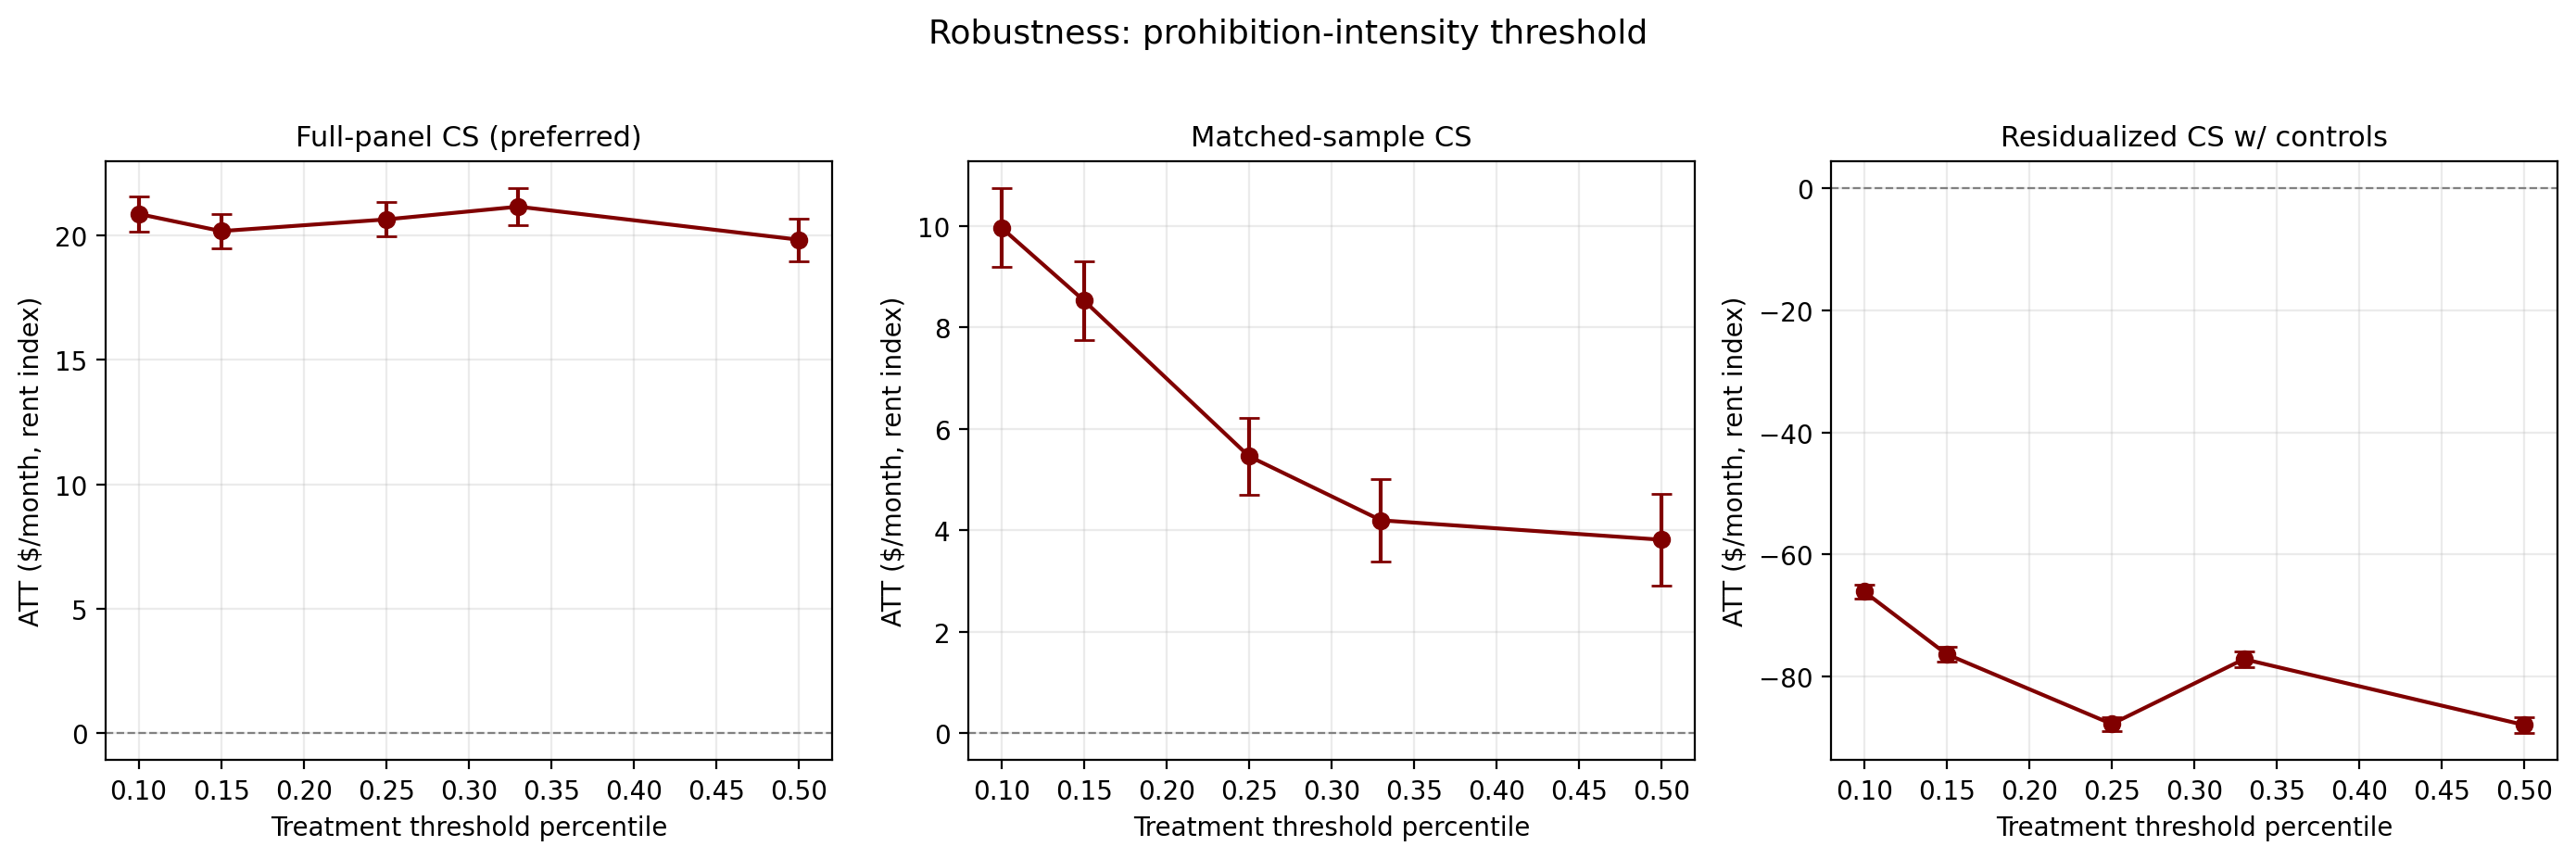
\includegraphics[width=0.92\linewidth]{threshold_percentile_att_by_spec.png}
  \caption{Pooled ATT by treatment-intensity percentile.}
  \label{fig:annex-pct-att}
\end{figure}

\textbf{Interpretation.} Matched ATTs are sensitive to how stringently ``treatment'' is defined: looser intensity cutoffs (lower $p$) associate with larger positive matched estimates, while stricter cutoffs shrink the treated set toward high-intensity tracts and reduce matched ATTs.
This pattern is consistent with heterogeneous exposure rather than proof of a stable causal magnitude; it motivates reporting the $p=0.25$ rule as a middle-ground intensity definition rather than as a uniquely identified effect size.

\textbf{Decision.} The preferred intensity cutoff remains $p=0.25$.

---

\section{Robustness overview}\label{app:robustness-overview}

\section{Cohort-specific results}\label{app:cohort-att}

Matched-sample Callaway--Sant'Anna group--time effects decompose by first-treatment cohort (adoption month).
Table~\ref{tab:annex-cohort-att} reports pooled post-period ATTs per cohort under the \textbf{intensity-threshold} rule (Appendix~\ref{app:treatment-intensity}); Table~\ref{tab:annex-cohort-att-binary} repeats the exercise under a \textbf{binary} first-prohibition definition.

\textbf{Pre-violations} counts significant pre-period coefficients among relative times $t\in\{-12,\ldots,-2\}$ (11 periods; $t=-1$ is the reference).
\textbf{Clean} cohorts have at most two such violations.
Early 2016 adoption months have small matched samples and wide confidence bands in the cohort event-study figures (Figures~\ref{fig:cohort-dynamics-p1}--\ref{fig:cohort-dynamics-p2}); they contribute noise to the aggregate V-shape but should not anchor policy conclusions.

The \textbf{2019-10} cohort (highlighted) tends to show flatter pre-treatment dynamics and a positive post-period path in the matched event-study panels; treat any cohort-specific magnitude as illustrative rather than as a standalone causal headline.

\begin{table}[htbp]
  \centering
  \caption{Cohort pooled post-period ATTs (intensity threshold, $p=0.25$, matched $k=3$).}
  \label{tab:annex-cohort-att}
  \small
  \input{../../output/did-cs-whitepaper-threshold/tables/tab_cohort_att.tex}
\end{table}

\begin{table}[htbp]
  \centering
  \caption{Cohort pooled post-period ATTs (binary treatment; matched $k=3$).}
  \label{tab:annex-cohort-att-binary}
  \small
  \input{../../output/did-cs-whitepaper-binary/tables/tab_cohort_att.tex}
\end{table}

\subsection{Calendar-month fixed effects (diagnostic)}\label{app:seasonality}

To probe whether $\sim$12-month oscillation in cohort panels reflects seasonal rent cycles, we re-estimate matched CS after subtracting panel-wide month-of-year means from rents (common calendar-month FE).
Table~\ref{tab:annex-seasonality} and Figures~\ref{fig:annex-seasonality-p1}--\ref{fig:annex-seasonality-p2} summarize the comparison.
In the May 2026 diagnostic run, calendar-month demeaning leaves the pooled matched ATT unchanged (about \$5.5/month) and does not reduce 2019-10 pre-trend violations (2 of 11 pre-periods significant under both specs).
We therefore \textbf{do not} adopt month-of-year adjustment in the headline rent-level specification.

\begin{table}[htbp]
  \centering
  \caption{Raw vs calendar-month demeaned matched CS (diagnostic).}
  \label{tab:annex-seasonality}
  \small
  % Auto-generated
\begin{tabular}{@{} l r r r r @{}}
\toprule
Spec & ATT (\$/mo.) & SE & Pre-trend $p$ & 2019-10 pre-viol. \\
\midrule
Raw & 5.5 & (0.39) & 0.000 & 2 \\
Month demeaned & 5.5 & (0.39) & 0.000 & 2 \\
\bottomrule
\end{tabular}

\end{table}

\IfFileExists{../../docs/robustness/figures/did_cohort_dynamics_seasonality_compare_p1.png}{%
\begin{figure}[p]
  \centering
  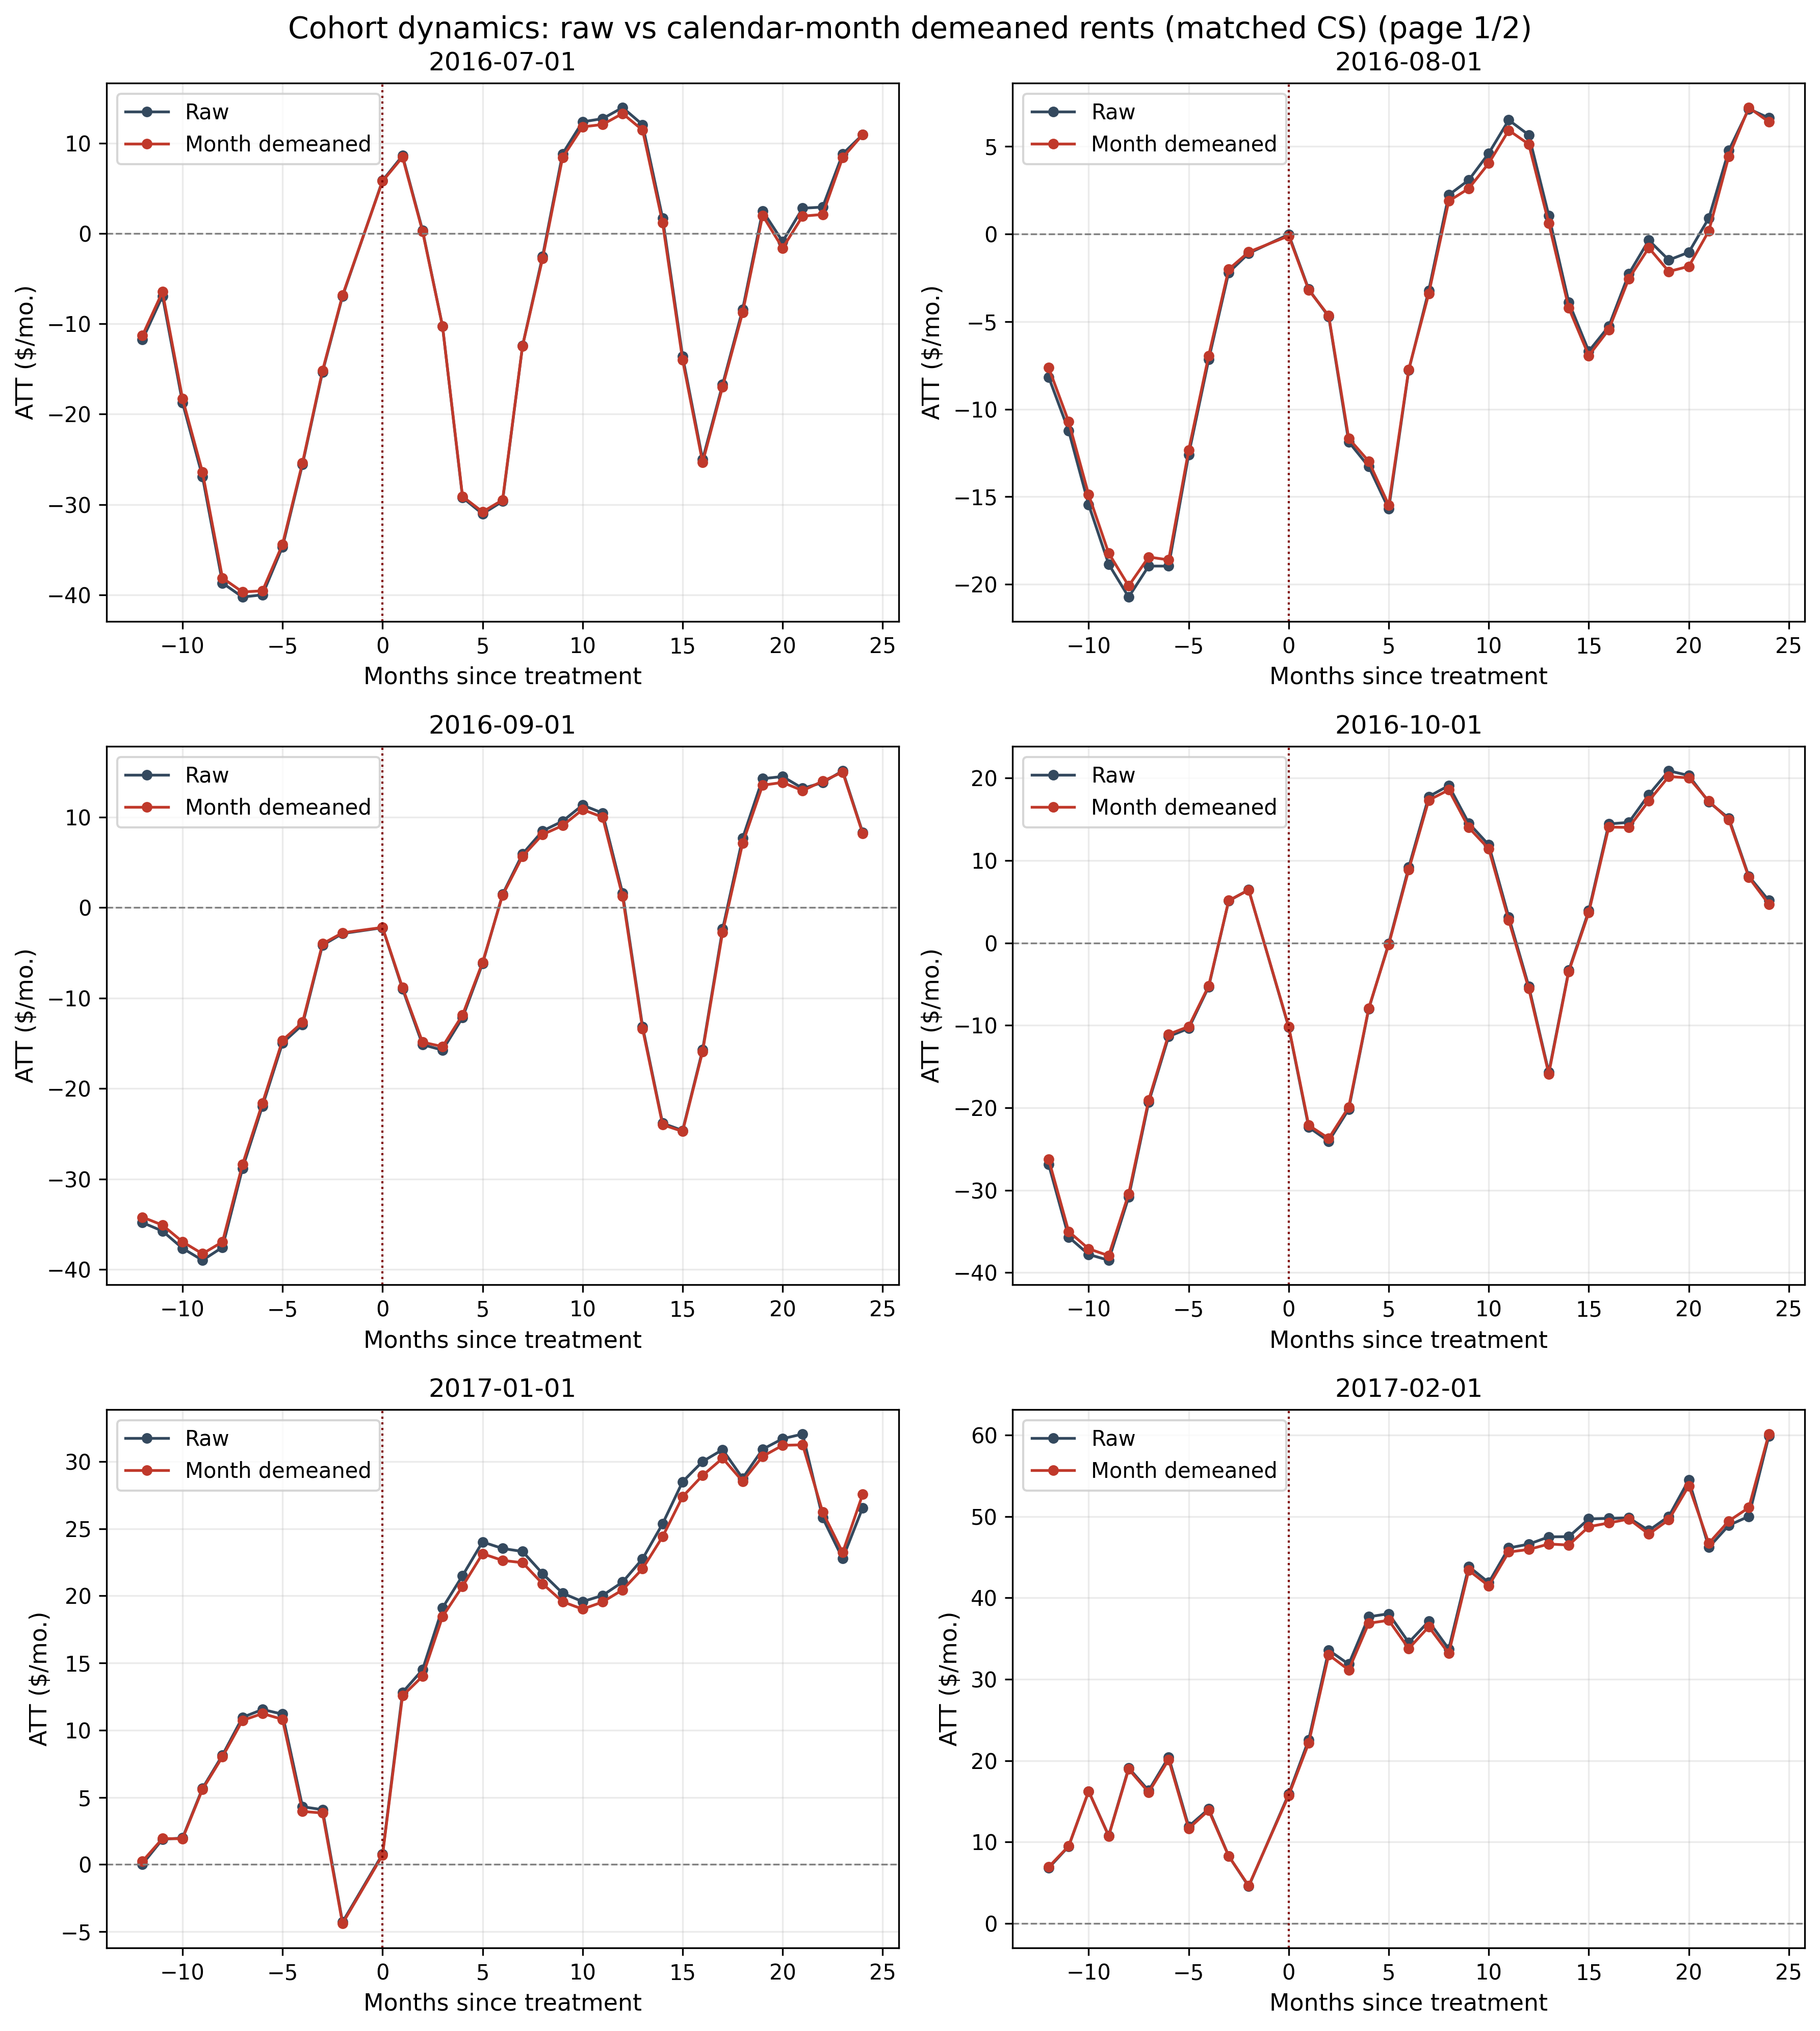
\includegraphics[width=0.92\linewidth]{did_cohort_dynamics_seasonality_compare_p1.png}
  \caption{Cohort dynamics: raw rents vs.\ month-of-year demeaned (matched CS), cohorts 1--6.}
  \figurenotes{Gray line: raw ZORI levels; red line: rents after subtracting panel-wide calendar-month means (common month FE). If seasonality drove pre-trends, demeaned paths should flatten before month 0; pooled ATT in Table~\ref{tab:annex-seasonality} is essentially unchanged.}
  \label{fig:annex-seasonality-p1}
\end{figure}

\begin{figure}[p]
  \centering
  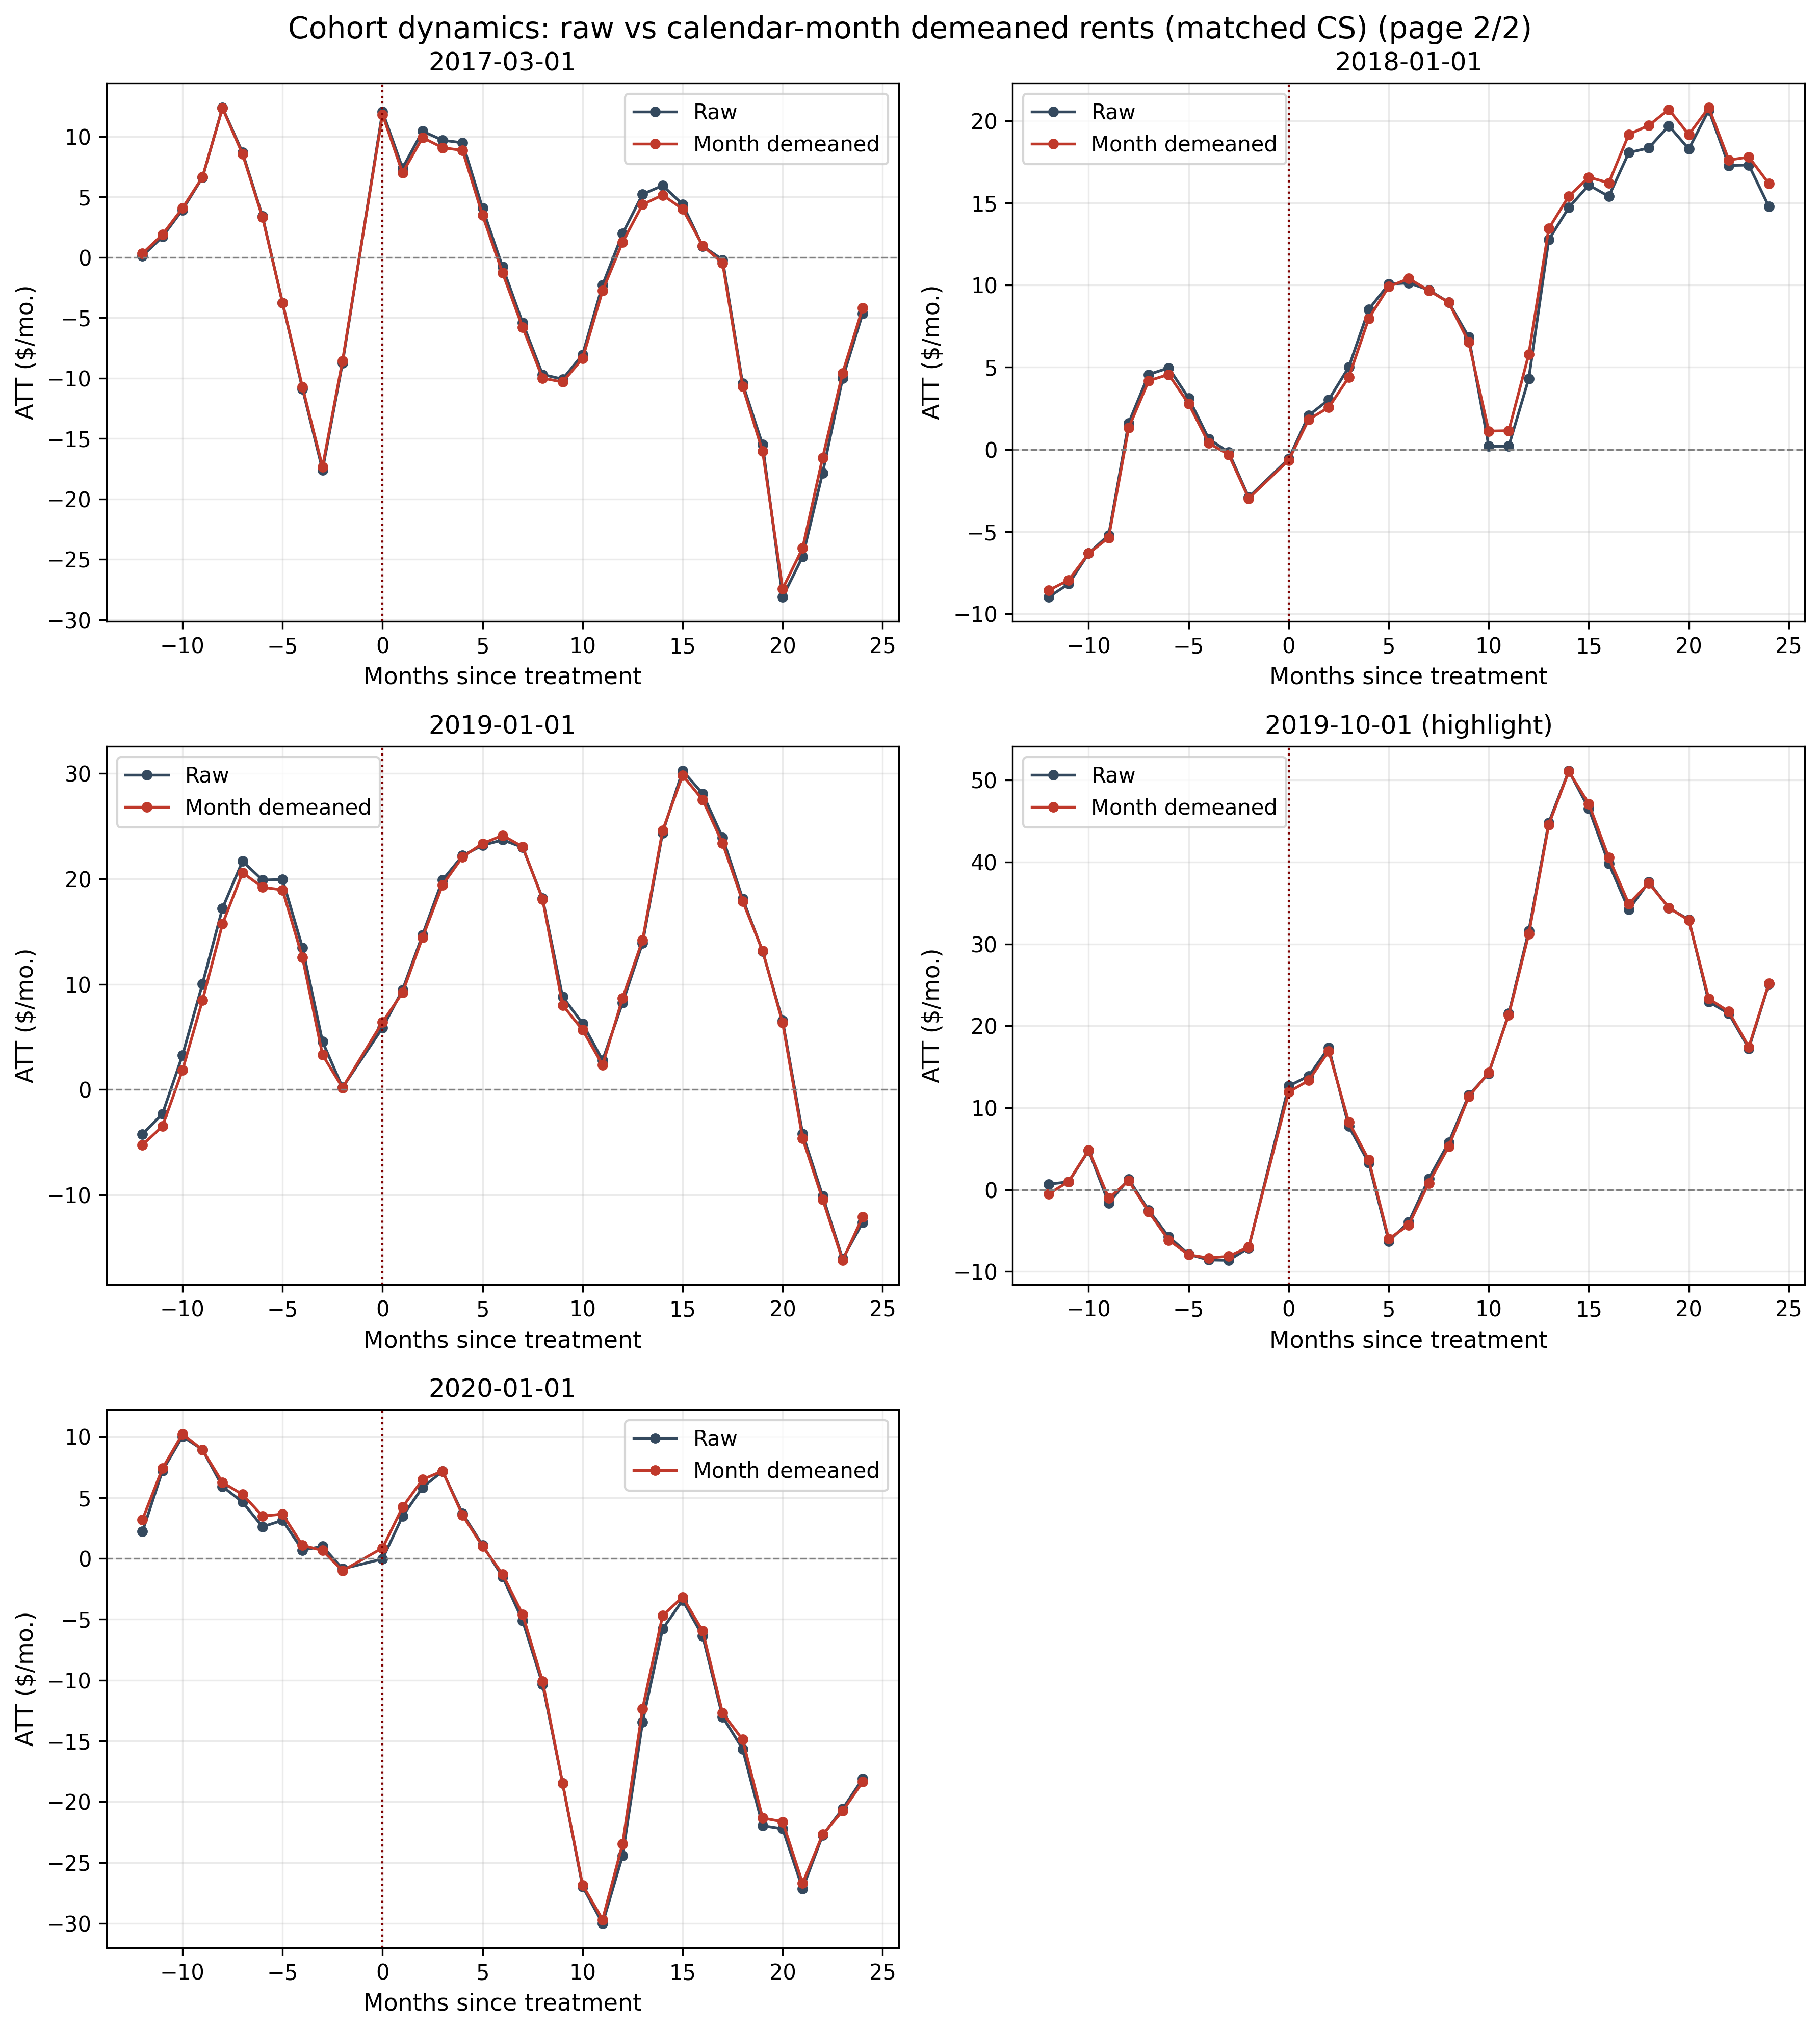
\includegraphics[width=0.92\linewidth]{did_cohort_dynamics_seasonality_compare_p2.png}
  \caption{Cohort dynamics: raw vs.\ demeaned (continued), cohorts 7--11.}
  \figurenotes{Same diagnostic as Figure~\ref{fig:annex-seasonality-p1}; 2019-10 cohort highlighted in the seasonality run when present on this page.}
  \label{fig:annex-seasonality-p2}
\end{figure}
}{%
\begin{figure}[p]
  \centering
  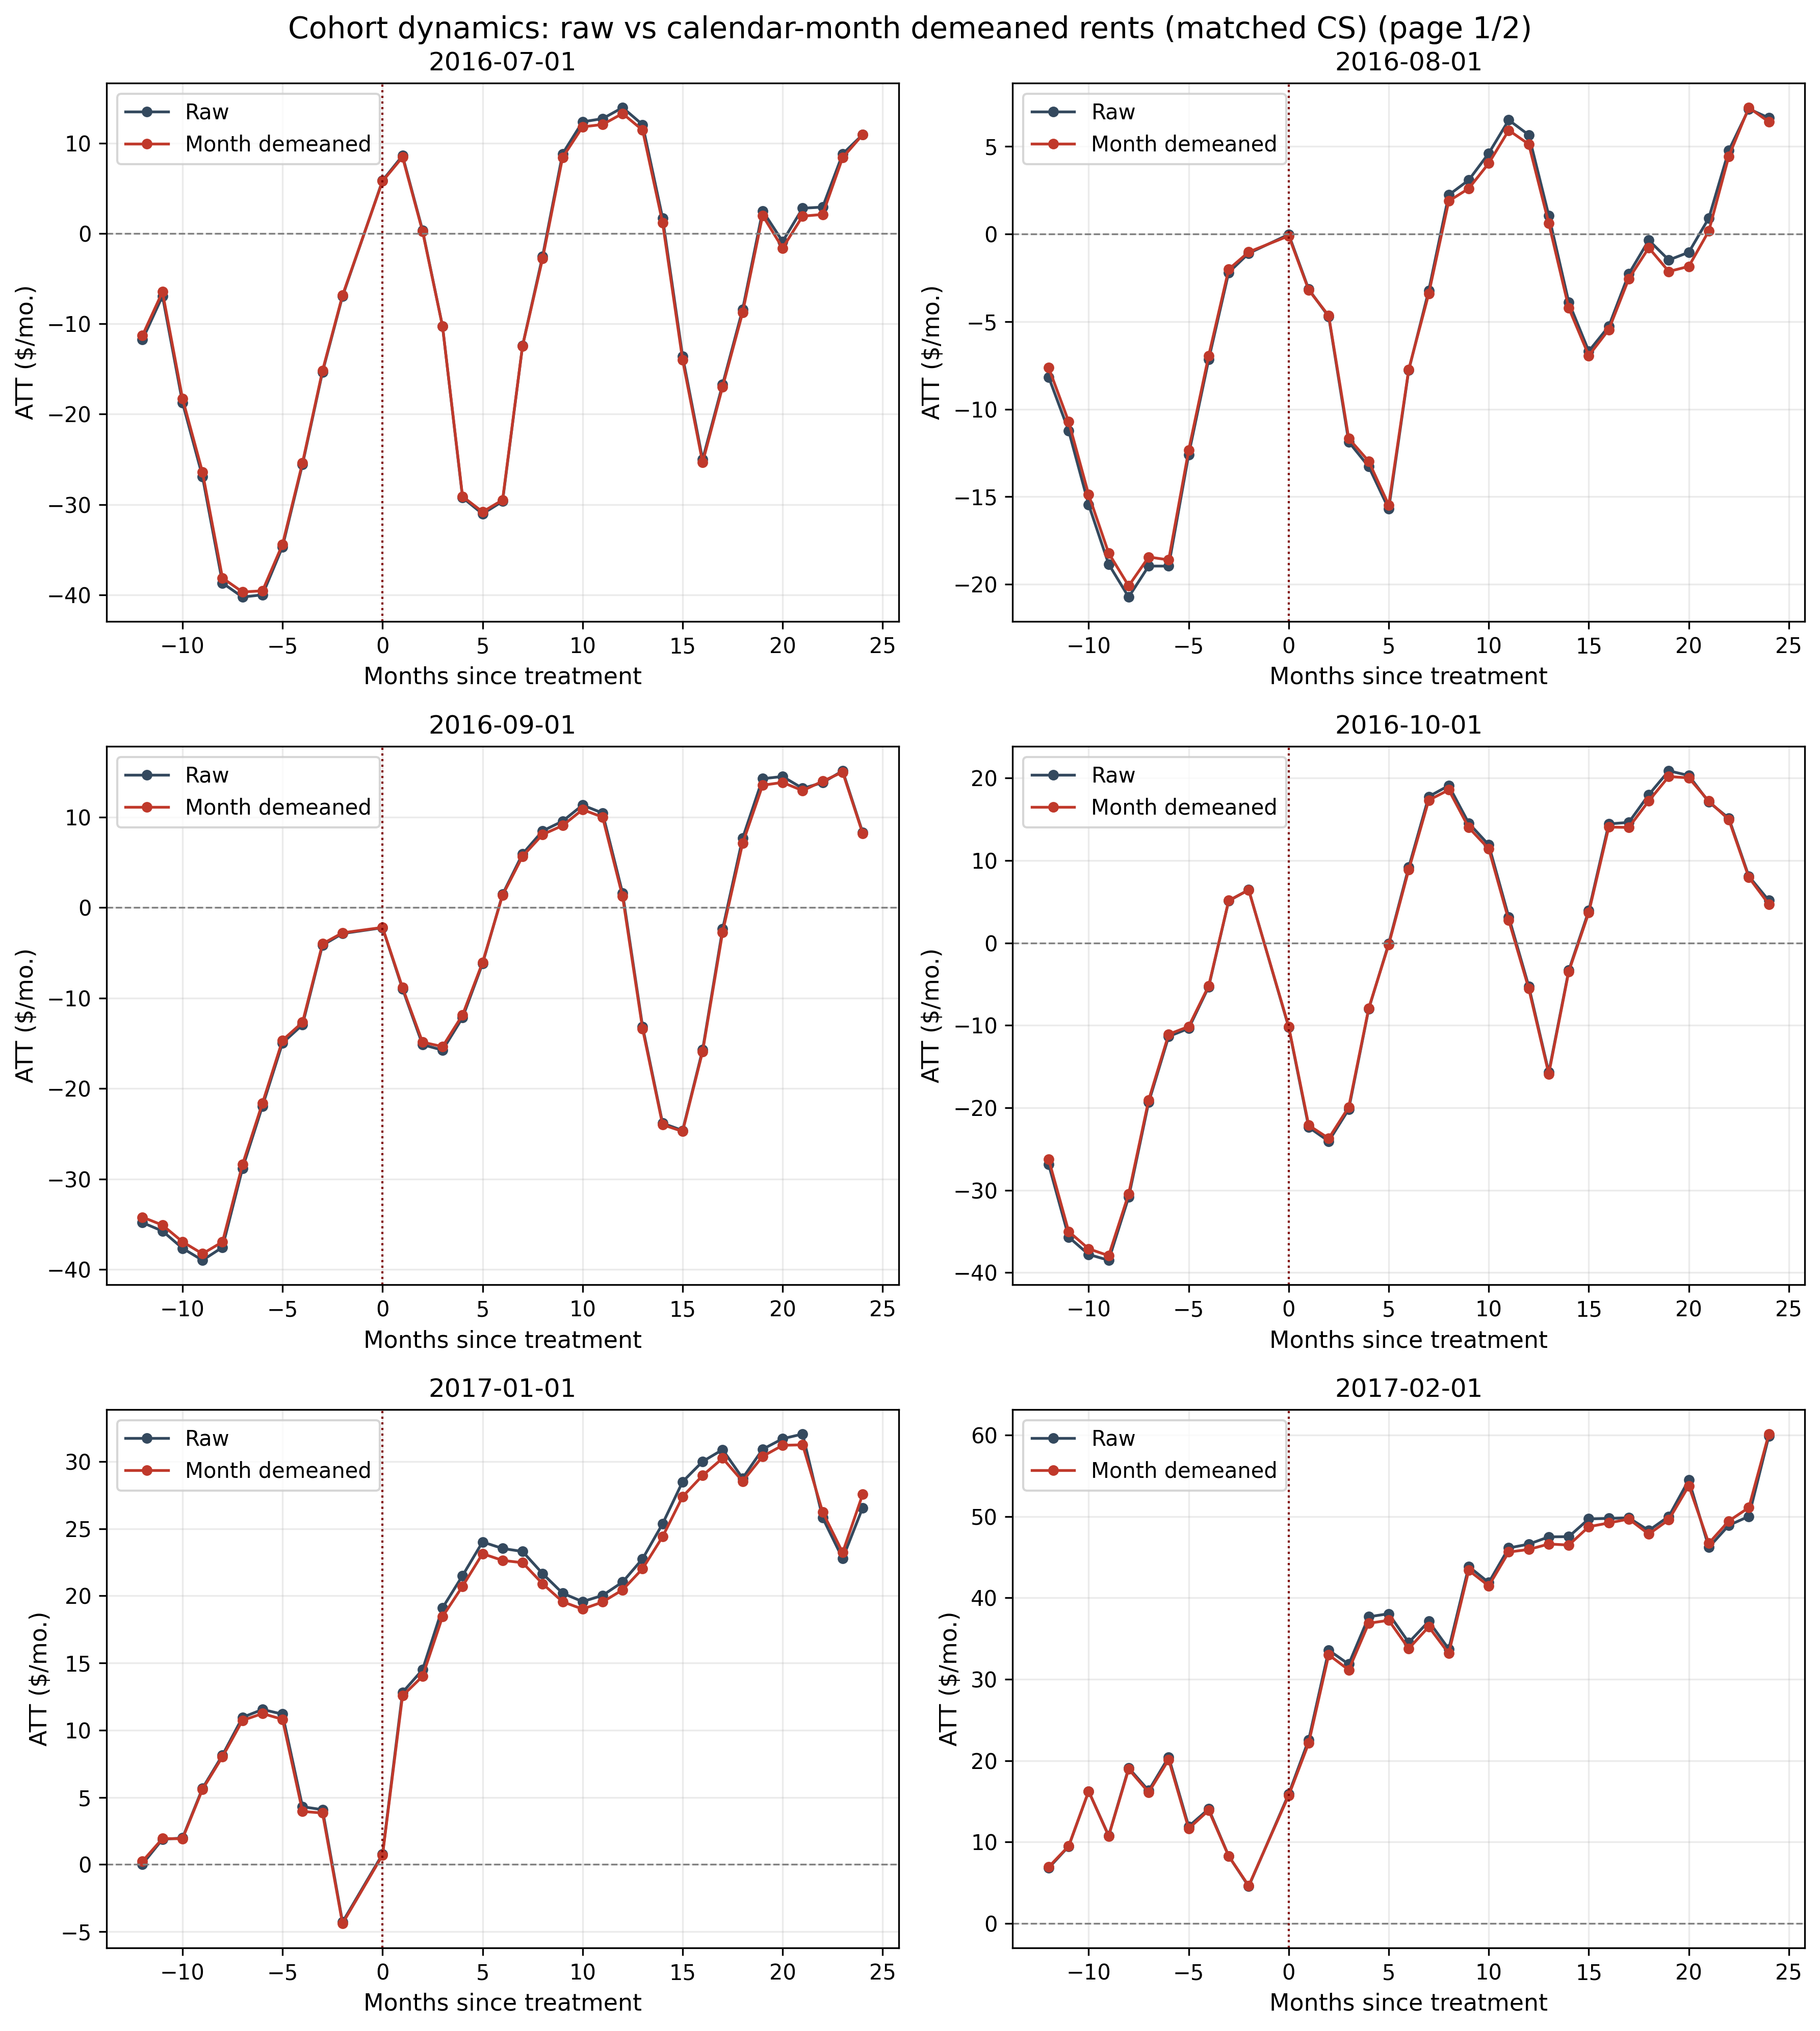
\includegraphics[width=0.88\linewidth]{did_cohort_dynamics_seasonality_compare.png}
  \caption{Cohort dynamics: raw rents vs.\ month-of-year demeaned (matched CS).}
  \figurenotes{Re-run \texttt{run\_seasonality\_diagnostic.py} to emit paginated appendix figures (\texttt{*\_p1.png}, \texttt{*\_p2.png}). Gray = raw ZORI; red = month-demeaned rents.}
  \label{fig:annex-seasonality}
\end{figure}
}%

---

\section{Parallel trends and residualized specifications}\label{app:parallel-trends}

\subsection{V-shaped pre-treatment dynamics}

Full-panel CS event-study coefficients relative to $t=-1$ exhibit a V-shaped pre-ban path: about $-$8/month at $t=-12$, a minimum near $-$16/month at $t=-8$, and recovery toward zero at $t=-1$.
A joint Wald test on pre-period group--time ATTs rejects a flat pre-trend null ($p<0.001$).
Treated tracts had higher pre-ban rent levels and faster growth than never-treated tracts---consistent with gentrification pressure in neighborhoods where prohibitions cluster.

\subsection{Why raw and residualized pooled ATTs diverge}

Positive full-panel and matched raw ATTs may partly reflect continuation of pre-ban reconvergence rather than a prohibition-caused rent increase.
Residualized CS with tract-linear trends fit on pre-ban months can \emph{over-extrapolate} the late recovery phase of the V-shape, producing large negative pooled ATTs on a preconditioned scale (about $-$88/month linear; even more extreme under quadratic detrend in Figure~\ref{fig:annex-quadratic}).

Neither sign should headline a rent-level policy conclusion without acknowledging the pre-trend violation.

\subsection{Pretrend heuristic (not HonestDiD)}

Table~\ref{tab:annex-honest-pretrends} summarizes a lightweight diagnostic exported alongside the whitepaper run.
It flags the magnitude of pre-period TWFE coefficients and their second differences; it does \textbf{not} implement the full sensitivity analysis of \citet{rbs2023}.
Use it only as a companion to the CS joint Wald test and the event-study figure.

\begin{table}[htbp]
  \centering
  \caption{Pretrend heuristic summary (not Rambachan--Roth HonestDiD).}
  \label{tab:annex-honest-pretrends}
  \input{../../output/did-cs-whitepaper-threshold/tables/tab_honest_pretrends.tex}
\end{table}

\begin{figure}[htbp]
  \centering
  \includegraphics[width=0.92\linewidth]{did_callaway_santanna_event_study_quadratic_detrend.png}
  \caption{Residualized CS event study with quadratic tract-specific detrending (sensitivity).}
  \label{fig:annex-quadratic}
\end{figure}

\subsection{Residualized CS semantics}\label{app:residualized}

The residualized branch removes ACS covariates and tract-specific time trends estimated on pre-treatment months, then applies standard Callaway--Sant'Anna on the preconditioned outcome.
Pooled residualized ATTs are \textbf{not} interpretable as changes in observed monthly rent in \$/month comparable to raw CS.
They are reported only to document sensitivity to detrending functional form.

---

\section{Replication notes}\label{app:replication}

Results in this brief were generated with the project's staggered-DiD replication pipeline (Callaway--Sant'Anna, May 2026 whitepaper run).
Diagnostic tables exported alongside figures include pre-trend Wald tests, matching balance, sample lineage, and pretrend regression summaries.
Detailed command-line runbooks and version-pinned defaults are maintained in the project repository for clinic partners and are not reproduced here.


\bibliographystyle{plainnat}
% Path relative to this directory when running bibtex from docs/white-paper/
\bibliography{../../literature/references}

\end{document}
